\documentclass[12pt]{article}\usepackage[]{graphicx}\usepackage[]{color}
% maxwidth is the original width if it is less than linewidth
% otherwise use linewidth (to make sure the graphics do not exceed the margin)
\makeatletter
\def\maxwidth{ %
  \ifdim\Gin@nat@width>\linewidth
    \linewidth
  \else
    \Gin@nat@width
  \fi
}
\makeatother

\definecolor{fgcolor}{rgb}{0.345, 0.345, 0.345}
\newcommand{\hlnum}[1]{\textcolor[rgb]{0.686,0.059,0.569}{#1}}%
\newcommand{\hlstr}[1]{\textcolor[rgb]{0.192,0.494,0.8}{#1}}%
\newcommand{\hlcom}[1]{\textcolor[rgb]{0.678,0.584,0.686}{\textit{#1}}}%
\newcommand{\hlopt}[1]{\textcolor[rgb]{0,0,0}{#1}}%
\newcommand{\hlstd}[1]{\textcolor[rgb]{0.345,0.345,0.345}{#1}}%
\newcommand{\hlkwa}[1]{\textcolor[rgb]{0.161,0.373,0.58}{\textbf{#1}}}%
\newcommand{\hlkwb}[1]{\textcolor[rgb]{0.69,0.353,0.396}{#1}}%
\newcommand{\hlkwc}[1]{\textcolor[rgb]{0.333,0.667,0.333}{#1}}%
\newcommand{\hlkwd}[1]{\textcolor[rgb]{0.737,0.353,0.396}{\textbf{#1}}}%
\let\hlipl\hlkwb

\usepackage{framed}
\makeatletter
\newenvironment{kframe}{%
 \def\at@end@of@kframe{}%
 \ifinner\ifhmode%
  \def\at@end@of@kframe{\end{minipage}}%
  \begin{minipage}{\columnwidth}%
 \fi\fi%
 \def\FrameCommand##1{\hskip\@totalleftmargin \hskip-\fboxsep
 \colorbox{shadecolor}{##1}\hskip-\fboxsep
     % There is no \\@totalrightmargin, so:
     \hskip-\linewidth \hskip-\@totalleftmargin \hskip\columnwidth}%
 \MakeFramed {\advance\hsize-\width
   \@totalleftmargin\z@ \linewidth\hsize
   \@setminipage}}%
 {\par\unskip\endMakeFramed%
 \at@end@of@kframe}
\makeatother

\definecolor{shadecolor}{rgb}{.97, .97, .97}
\definecolor{messagecolor}{rgb}{0, 0, 0}
\definecolor{warningcolor}{rgb}{1, 0, 1}
\definecolor{errorcolor}{rgb}{1, 0, 0}
\newenvironment{knitrout}{}{} % an empty environment to be redefined in TeX

\usepackage{alltt}
 
\usepackage[margin=1in]{geometry}
\usepackage{amsmath,amsthm,amssymb, mathtools}
\usepackage[T1]{fontenc}
\usepackage{lmodern}
\usepackage{fixltx2e}
\usepackage[shortlabels]{enumitem}
 
\newcommand{\N}{\mathbb{N}}
\newcommand{\R}{\mathbb{R}}
\newcommand{\Z}{\mathbb{Z}}
\newcommand{\Q}{\mathbb{Q}}

\newenvironment{theorem}[2][Theorem]{\begin{trivlist}
\item[\hskip \labelsep {\bfseries #1}\hskip \labelsep {\bfseries #2.}]}{\end{trivlist}}
\newenvironment{lemma}[2][Lemma]{\begin{trivlist}
\item[\hskip \labelsep {\bfseries #1}\hskip \labelsep {\bfseries #2.}]}{\end{trivlist}}
\newenvironment{exercise}[2][Exercise]{\begin{trivlist}
\item[\hskip \labelsep {\bfseries #1}\hskip \labelsep {\bfseries #2.}]}{\end{trivlist}}
\newenvironment{problem}[2][Problem]{\begin{trivlist}
\item[\hskip \labelsep {\bfseries #1}\hskip \labelsep {\bfseries #2.}]}{\end{trivlist}}
\newenvironment{question}[2][Question]{\begin{trivlist}
\item[\hskip \labelsep {\bfseries #1}\hskip \labelsep {\bfseries #2.}]}{\end{trivlist}}
\newenvironment{corollary}[2][Corollary]{\begin{trivlist}
\item[\hskip \labelsep {\bfseries #1}\hskip \labelsep {\bfseries #2.}]}{\end{trivlist}}
\newcommand{\textfrac}[2]{\dfrac{\text{#1}}{\text{#2}}}
\IfFileExists{upquote.sty}{\usepackage{upquote}}{}
\begin{document}

\title{Ch. 7 - Moving Beyond Linearity}

\author{Chris Hayduk}
\date{\today}

\maketitle



\section{Polynomial Regression and Step Functions}

Polynomial regression and step functions both exist to give a more flexible fit than standard linear regression will allow. Polynomial regression works by creating new variables out of powers of the initial prediction variable. For example, if the initial predictor is $x$, we may use $x, x^2$, and $x^3$ as our three predictors if we wish to use a cubic fit. On the other than, step functions work by cutitng the data up into bins and then fitting constant functions on each of these bins.\\

We start here by fitting a degree 4 polynomial with the \texttt{lm()} function.

\begin{knitrout}
\definecolor{shadecolor}{rgb}{0.969, 0.969, 0.969}\color{fgcolor}\begin{kframe}
\begin{alltt}
\hlkwd{data}\hlstd{(Wage)}
\hlkwd{attach}\hlstd{(Wage)}
\hlstd{fit}\hlkwb{=}\hlkwd{lm}\hlstd{(wage}\hlopt{~}\hlkwd{poly}\hlstd{(age,}\hlnum{4}\hlstd{),} \hlkwc{data}\hlstd{=Wage)}
\hlkwd{coef}\hlstd{(}\hlkwd{summary}\hlstd{(fit))}
\end{alltt}
\begin{verbatim}
##                 Estimate Std. Error    t value     Pr(>|t|)
## (Intercept)    111.70361  0.7287409 153.283015 0.000000e+00
## poly(age, 4)1  447.06785 39.9147851  11.200558 1.484604e-28
## poly(age, 4)2 -478.31581 39.9147851 -11.983424 2.355831e-32
## poly(age, 4)3  125.52169 39.9147851   3.144742 1.678622e-03
## poly(age, 4)4  -77.91118 39.9147851  -1.951938 5.103865e-02
\end{verbatim}
\end{kframe}
\end{knitrout}

The \texttt{poly()} function used above allows us to avoid writing out a long equation by hand. However, by default it returns a matrix whose columns are a basis of orthogonal polynomials. That is, each column is a linear combination of the variables $\text{age}, \text{age}^2, \text{age}^3$, and $\text{age}^4$. While the choice of basis will not affect the fitted values, we may want to use $\text{age}, \text{age}^2, \text{age}^3$, and $\text{age}^4$ directly. We can do this by setting \texttt{raw=TRUE} in the arguments for the function \texttt{poly()}.

\begin{knitrout}
\definecolor{shadecolor}{rgb}{0.969, 0.969, 0.969}\color{fgcolor}\begin{kframe}
\begin{alltt}
\hlstd{fit2}\hlkwb{=}\hlkwd{lm}\hlstd{(wage}\hlopt{~}\hlkwd{poly}\hlstd{(age,}\hlnum{4}\hlstd{,}\hlkwc{raw}\hlstd{=T),}\hlkwc{data}\hlstd{=Wage)}
\hlkwd{coef}\hlstd{(}\hlkwd{summary}\hlstd{(fit2))}
\end{alltt}
\begin{verbatim}
##                             Estimate   Std. Error   t value     Pr(>|t|)
## (Intercept)            -1.841542e+02 6.004038e+01 -3.067172 0.0021802539
## poly(age, 4, raw = T)1  2.124552e+01 5.886748e+00  3.609042 0.0003123618
## poly(age, 4, raw = T)2 -5.638593e-01 2.061083e-01 -2.735743 0.0062606446
## poly(age, 4, raw = T)3  6.810688e-03 3.065931e-03  2.221409 0.0263977518
## poly(age, 4, raw = T)4 -3.203830e-05 1.641359e-05 -1.951938 0.0510386498
\end{verbatim}
\end{kframe}
\end{knitrout}

There ae several other equivalent was of fitting this model in R. For example,

\begin{knitrout}
\definecolor{shadecolor}{rgb}{0.969, 0.969, 0.969}\color{fgcolor}\begin{kframe}
\begin{alltt}
\hlstd{fit2a} \hlkwb{=} \hlkwd{lm}\hlstd{(wage}\hlopt{~}\hlstd{age}\hlopt{+}\hlkwd{I}\hlstd{(age}\hlopt{^}\hlnum{2}\hlstd{)}\hlopt{+}\hlkwd{I}\hlstd{(age}\hlopt{^}\hlnum{3}\hlstd{)}\hlopt{+}\hlkwd{I}\hlstd{(age}\hlopt{^}\hlnum{4}\hlstd{),} \hlkwc{data}\hlstd{=Wage)}
\hlkwd{coef}\hlstd{(fit2a)}
\end{alltt}
\begin{verbatim}
##   (Intercept)           age      I(age^2)      I(age^3)      I(age^4) 
## -1.841542e+02  2.124552e+01 -5.638593e-01  6.810688e-03 -3.203830e-05
\end{verbatim}
\end{kframe}
\end{knitrout}

and,

\begin{knitrout}
\definecolor{shadecolor}{rgb}{0.969, 0.969, 0.969}\color{fgcolor}\begin{kframe}
\begin{alltt}
\hlstd{fit2b} \hlkwb{=} \hlkwd{lm}\hlstd{(wage}\hlopt{~}\hlkwd{cbind}\hlstd{(age, age}\hlopt{^}\hlnum{2}\hlstd{, age}\hlopt{^}\hlnum{3}\hlstd{, age}\hlopt{^}\hlnum{4}\hlstd{),} \hlkwc{data} \hlstd{= Wage)}
\end{alltt}
\end{kframe}
\end{knitrout}

We now create a grid of values for \texttt{age} at which we want predictions, and then call the generic \texttt{predict()} function, specifying that we want standard errors as well.

\begin{knitrout}
\definecolor{shadecolor}{rgb}{0.969, 0.969, 0.969}\color{fgcolor}\begin{kframe}
\begin{alltt}
\hlstd{agelims}\hlkwb{=}\hlkwd{range}\hlstd{(age)}
\hlstd{age.grid}\hlkwb{=}\hlkwd{seq}\hlstd{(}\hlkwc{from}\hlstd{=agelims[}\hlnum{1}\hlstd{],} \hlkwc{to} \hlstd{= agelims[}\hlnum{2}\hlstd{])}
\hlstd{preds}\hlkwb{=}\hlkwd{predict}\hlstd{(fit,} \hlkwc{newdata}\hlstd{=}\hlkwd{list}\hlstd{(}\hlkwc{age}\hlstd{=age.grid),} \hlkwc{se}\hlstd{=}\hlnum{TRUE}\hlstd{)}
\hlstd{se.bands} \hlkwb{=} \hlkwd{cbind}\hlstd{(preds}\hlopt{$}\hlstd{fit}\hlopt{+}\hlnum{2}\hlopt{*}\hlstd{preds}\hlopt{$}\hlstd{se.fit, preds}\hlopt{$}\hlstd{fit}\hlopt{-}\hlnum{2}\hlopt{*}\hlstd{preds}\hlopt{$}\hlstd{se.fit)}
\end{alltt}
\end{kframe}
\end{knitrout}

The above code creates our grid of age values, gets predictions for each value in the grid, and then sets the standard error bars at 95\% confidence (two times the standard error plus/minus the prediction). Finally, let us plot the data and add the fit from the degree-4 polynomial.

\begin{knitrout}
\definecolor{shadecolor}{rgb}{0.969, 0.969, 0.969}\color{fgcolor}\begin{kframe}
\begin{alltt}
\hlkwd{par}\hlstd{(}\hlkwc{mfrow}\hlstd{=}\hlkwd{c}\hlstd{(}\hlnum{1}\hlstd{,}\hlnum{1}\hlstd{),} \hlkwc{mar}\hlstd{=}\hlkwd{c}\hlstd{(}\hlnum{4.5}\hlstd{,}\hlnum{4.5}\hlstd{,}\hlnum{1}\hlstd{,}\hlnum{1}\hlstd{),} \hlkwc{oma}\hlstd{=}\hlkwd{c}\hlstd{(}\hlnum{0}\hlstd{,}\hlnum{0}\hlstd{,}\hlnum{4}\hlstd{,}\hlnum{0}\hlstd{))}
\hlkwd{plot}\hlstd{(age, wage,} \hlkwc{xlim}\hlstd{=agelims,} \hlkwc{cex}\hlstd{=}\hlnum{.5}\hlstd{,} \hlkwc{col}\hlstd{=}\hlstr{"darkgrey"}\hlstd{)}
\hlkwd{title}\hlstd{(}\hlstr{"Degree-4 Polynomial"}\hlstd{,} \hlkwc{outer}\hlstd{=T)}
\hlkwd{lines}\hlstd{(age.grid, preds}\hlopt{$}\hlstd{fit,} \hlkwc{lwd}\hlstd{=}\hlnum{2}\hlstd{,} \hlkwc{col}\hlstd{=}\hlstr{"blue"}\hlstd{)}
\hlkwd{matlines}\hlstd{(age.grid, se.bands,} \hlkwc{lwd}\hlstd{=}\hlnum{1}\hlstd{,} \hlkwc{col}\hlstd{=}\hlstr{"blue"}\hlstd{,} \hlkwc{lty}\hlstd{=}\hlnum{3}\hlstd{)}
\end{alltt}
\end{kframe}
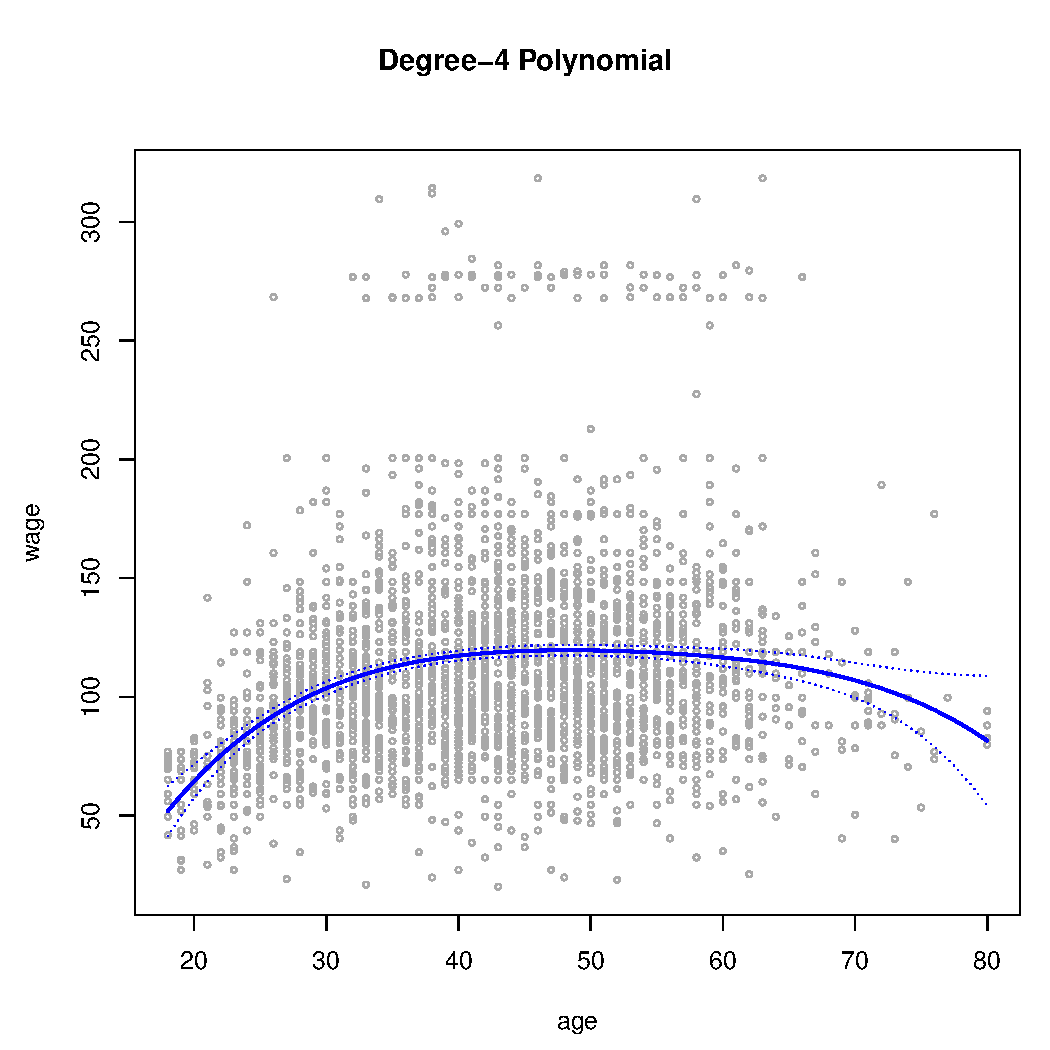
\includegraphics[width=\maxwidth]{figure/unnamed-chunk-7-1} 

\end{knitrout}

As we mentioned above, the choice of basis will not affect the fitted values of the function. We can verify this by checking the predicted values on our age grid from both types of our fitted polynomial functions:

\begin{knitrout}
\definecolor{shadecolor}{rgb}{0.969, 0.969, 0.969}\color{fgcolor}\begin{kframe}
\begin{alltt}
\hlstd{preds2} \hlkwb{=} \hlkwd{predict}\hlstd{(fit2,} \hlkwc{newdata}\hlstd{=}\hlkwd{list}\hlstd{(}\hlkwc{age}\hlstd{=age.grid),} \hlkwc{se}\hlstd{=}\hlnum{TRUE}\hlstd{)}
\hlkwd{max}\hlstd{(}\hlkwd{abs}\hlstd{(preds}\hlopt{$}\hlstd{fit}\hlopt{-}\hlstd{preds2}\hlopt{$}\hlstd{fit))}
\end{alltt}
\begin{verbatim}
## [1] 7.81597e-11
\end{verbatim}
\end{kframe}
\end{knitrout}

As we can see, the maximum of the absolute value of the difference of these two fits is extremely close to 0.\\

In practice, we will want to check several possible polynomial degrees in order to find the simplest model that provides the best fit. We will now fit models ranging from linear to degree-5 polynomials and use the \texttt{anova()} function to perform an analysis of variance in order to determine the best model. Analysis of variance (ANOVA) works by testing the null hypothesis that a model $M_1$ is sufficient to explain the data again the alternative hypothesis that a more complex model $M_2$ is required. In order to use the \texttt{anova()} function, $M_1$ and $M_2$ must be nested models. In this case, we are fitting five different models and wll sequentially compare the simpler model to the more complex model.

\begin{knitrout}
\definecolor{shadecolor}{rgb}{0.969, 0.969, 0.969}\color{fgcolor}\begin{kframe}
\begin{alltt}
\hlstd{fit.1} \hlkwb{=} \hlkwd{lm}\hlstd{(wage}\hlopt{~}\hlstd{age,} \hlkwc{data}\hlstd{=Wage)}
\hlstd{fit.2} \hlkwb{=} \hlkwd{lm}\hlstd{(wage}\hlopt{~}\hlkwd{poly}\hlstd{(age,}\hlnum{2}\hlstd{),} \hlkwc{data}\hlstd{=Wage)}
\hlstd{fit.3} \hlkwb{=} \hlkwd{lm}\hlstd{(wage}\hlopt{~}\hlkwd{poly}\hlstd{(age,}\hlnum{3}\hlstd{),} \hlkwc{data}\hlstd{=Wage)}
\hlstd{fit.4} \hlkwb{=} \hlkwd{lm}\hlstd{(wage}\hlopt{~}\hlkwd{poly}\hlstd{(age,}\hlnum{4}\hlstd{),} \hlkwc{data}\hlstd{=Wage)}
\hlstd{fit.5} \hlkwb{=} \hlkwd{lm}\hlstd{(wage}\hlopt{~}\hlkwd{poly}\hlstd{(age,}\hlnum{5}\hlstd{),} \hlkwc{data}\hlstd{=Wage)}
\hlkwd{anova}\hlstd{(fit.1, fit.2, fit.3, fit.4, fit.5)}
\end{alltt}
\begin{verbatim}
## Analysis of Variance Table
## 
## Model 1: wage ~ age
## Model 2: wage ~ poly(age, 2)
## Model 3: wage ~ poly(age, 3)
## Model 4: wage ~ poly(age, 4)
## Model 5: wage ~ poly(age, 5)
##   Res.Df     RSS Df Sum of Sq        F    Pr(>F)    
## 1   2998 5022216                                    
## 2   2997 4793430  1    228786 143.5931 < 2.2e-16 ***
## 3   2996 4777674  1     15756   9.8888  0.001679 ** 
## 4   2995 4771604  1      6070   3.8098  0.051046 .  
## 5   2994 4770322  1      1283   0.8050  0.369682    
## ---
## Signif. codes:  0 '***' 0.001 '**' 0.01 '*' 0.05 '.' 0.1 ' ' 1
\end{verbatim}
\end{kframe}
\end{knitrout}

The p-value comparing the linear Model 1 to the quadratic Model 2 is essentially 0, indicating that a linear fit is not sufficient. Similarly, the p-value comparing the quadratic Model 2 to the cubic Model 3 is very low, so the quadratic fit is also insufficient. The p-value comparing the cubic model and the degree-4 polynomial is approximately 5\%, while the degree-5 polynomial seems unnecessary because its p-value is 0.37. Hence, either a cubic or quartic polynomial appears to provide a reasonable fit to the data, but lower- or higher-order models are not justified.\\

We can actually avoid using the \texttt{anova()} function since \texttt{poly()} creates orthogonal polynomials:

\begin{knitrout}
\definecolor{shadecolor}{rgb}{0.969, 0.969, 0.969}\color{fgcolor}\begin{kframe}
\begin{alltt}
\hlkwd{coef}\hlstd{(}\hlkwd{summary}\hlstd{(fit.5))}
\end{alltt}
\begin{verbatim}
##                 Estimate Std. Error     t value     Pr(>|t|)
## (Intercept)    111.70361  0.7287647 153.2780243 0.000000e+00
## poly(age, 5)1  447.06785 39.9160847  11.2001930 1.491111e-28
## poly(age, 5)2 -478.31581 39.9160847 -11.9830341 2.367734e-32
## poly(age, 5)3  125.52169 39.9160847   3.1446392 1.679213e-03
## poly(age, 5)4  -77.91118 39.9160847  -1.9518743 5.104623e-02
## poly(age, 5)5  -35.81289 39.9160847  -0.8972045 3.696820e-01
\end{verbatim}
\end{kframe}
\end{knitrout}

As you can see, the p-values aree exactly the same, and in fact the square of the t-statistics are equal to the F-statistics from the \texttt{anova()} function. However, the ANOVA method works whether or not we used orthogonal polynomials; it also works when we have other terms in the model as well. For example, we can use \texttt{anova()} to compare these three models:

\begin{knitrout}
\definecolor{shadecolor}{rgb}{0.969, 0.969, 0.969}\color{fgcolor}\begin{kframe}
\begin{alltt}
\hlstd{fit.1} \hlkwb{=} \hlkwd{lm}\hlstd{(wage}\hlopt{~}\hlstd{education}\hlopt{+}\hlstd{age,} \hlkwc{data}\hlstd{=Wage)}
\hlstd{fit.2} \hlkwb{=} \hlkwd{lm}\hlstd{(wage}\hlopt{~}\hlstd{education} \hlopt{+} \hlkwd{poly}\hlstd{(age,}\hlnum{2}\hlstd{),} \hlkwc{data}\hlstd{=Wage)}
\hlstd{fit.3} \hlkwb{=} \hlkwd{lm}\hlstd{(wage}\hlopt{~}\hlstd{education}\hlopt{+}\hlkwd{poly}\hlstd{(age,}\hlnum{3}\hlstd{),} \hlkwc{data}\hlstd{=Wage)}
\hlkwd{anova}\hlstd{(fit.1, fit.2, fit.3)}
\end{alltt}
\begin{verbatim}
## Analysis of Variance Table
## 
## Model 1: wage ~ education + age
## Model 2: wage ~ education + poly(age, 2)
## Model 3: wage ~ education + poly(age, 3)
##   Res.Df     RSS Df Sum of Sq        F Pr(>F)    
## 1   2994 3867992                                 
## 2   2993 3725395  1    142597 114.6969 <2e-16 ***
## 3   2992 3719809  1      5587   4.4936 0.0341 *  
## ---
## Signif. codes:  0 '***' 0.001 '**' 0.01 '*' 0.05 '.' 0.1 ' ' 1
\end{verbatim}
\end{kframe}
\end{knitrout}

As an alternative to using ANOVA, we could also choose the polynomial degree using cross-validation.\\

Now let us consider the task of predicting whether an individual earns more than \$250,000 per year. We proceed much as before, except that first we create the appropriate response vector, and then apply the \texttt{glm()} function using \texttt{family=''binomial``} in order to fit a polynomial logistic regression model.

\begin{knitrout}
\definecolor{shadecolor}{rgb}{0.969, 0.969, 0.969}\color{fgcolor}\begin{kframe}
\begin{alltt}
\hlstd{fit} \hlkwb{=} \hlkwd{glm}\hlstd{(}\hlkwd{I}\hlstd{(wage}\hlopt{>}\hlnum{250}\hlstd{)} \hlopt{~} \hlkwd{poly}\hlstd{(age,}\hlnum{4}\hlstd{),} \hlkwc{data} \hlstd{= Wage,} \hlkwc{family} \hlstd{= binomial)}
\end{alltt}
\end{kframe}
\end{knitrout}

We are using the wrapper \texttt{I()} to create the binary response variable on the fly. The expression \texttt{wage>250} evaluates to a logical vairable containing \texttt{TRUEs} and \texttt{FALSEs}, which \texttt{glm()} coerces to binary by setting \texttt{TRUEs} to $1$ and \texttt{FALSEs} to $0$.\\

We now use the \texttt{predict()} function to make our predictions,
\begin{knitrout}
\definecolor{shadecolor}{rgb}{0.969, 0.969, 0.969}\color{fgcolor}\begin{kframe}
\begin{alltt}
\hlstd{preds}\hlkwb{=}\hlkwd{predict}\hlstd{(fit,} \hlkwc{newdata}\hlstd{=}\hlkwd{list}\hlstd{(}\hlkwc{age}\hlstd{=age.grid),}\hlkwc{se}\hlstd{=T)}
\end{alltt}
\end{kframe}
\end{knitrout}

Confidence intervals in this scenario are a bit more involved than they were in the linear regression case. Our predictions are for the \textit{logit}. That is, we have fit a model of the form $$\log \left(\frac{\text{Pr}(Y=1|X)}{1 - \text{Pr}(Y=1|X)}\right) = X\beta$$, and the predictions given are of the form $X\hat{\beta}$. The standard errors given are also of this form. In order to obtain confidence intervals for $\text{Pr}(Y=1|X)$, we use the transformation $$\text{Pr}(Y=1|X) = \frac{\exp(X\beta)}{1 + \exp(X\beta)}$$

\begin{knitrout}
\definecolor{shadecolor}{rgb}{0.969, 0.969, 0.969}\color{fgcolor}\begin{kframe}
\begin{alltt}
\hlstd{pfit} \hlkwb{=} \hlkwd{exp}\hlstd{(preds}\hlopt{$}\hlstd{fit)}\hlopt{/}\hlstd{(}\hlnum{1}\hlopt{+}\hlkwd{exp}\hlstd{(preds}\hlopt{$}\hlstd{fit))}
\hlstd{se.bands.logit} \hlkwb{=} \hlkwd{cbind}\hlstd{(preds}\hlopt{$}\hlstd{fit}\hlopt{+}\hlnum{2}\hlopt{*}\hlstd{preds}\hlopt{$}\hlstd{se.fit, preds}\hlopt{$}\hlstd{fit}\hlopt{-}\hlnum{2}\hlopt{*}\hlstd{preds}\hlopt{$}\hlstd{se.fit)}
\hlstd{se.bands} \hlkwb{=} \hlkwd{exp}\hlstd{(se.bands.logit)}\hlopt{/}\hlstd{(}\hlnum{1}\hlopt{+}\hlkwd{exp}\hlstd{(se.bands.logit))}
\end{alltt}
\end{kframe}
\end{knitrout}

However, the corresponding confidence intervals would not have been sensible because we would end up with negative probabilities! Finally, the right-hand plot from Figure 7.1 was made as follows:

\begin{knitrout}
\definecolor{shadecolor}{rgb}{0.969, 0.969, 0.969}\color{fgcolor}\begin{kframe}
\begin{alltt}
\hlkwd{plot}\hlstd{(age,}\hlkwd{I}\hlstd{(wage}\hlopt{>}\hlnum{250}\hlstd{),} \hlkwc{xlim}\hlstd{=agelims,} \hlkwc{type}\hlstd{=}\hlstr{"n"}\hlstd{,} \hlkwc{ylim}\hlstd{=}\hlkwd{c}\hlstd{(}\hlnum{0}\hlstd{,}\hlnum{0.2}\hlstd{))}
\hlkwd{points}\hlstd{(}\hlkwd{jitter}\hlstd{(age),} \hlkwd{I}\hlstd{((wage}\hlopt{>}\hlnum{250}\hlstd{)}\hlopt{/}\hlnum{5}\hlstd{),} \hlkwc{cex}\hlstd{=}\hlnum{.5}\hlstd{,} \hlkwc{pch}\hlstd{=}\hlstr{"|"}\hlstd{,} \hlkwc{col}\hlstd{=}\hlstr{"darkgrey"}\hlstd{)}
\hlkwd{lines}\hlstd{(age.grid, pfit,} \hlkwc{lwd}\hlstd{=}\hlnum{2}\hlstd{,} \hlkwc{col}\hlstd{=}\hlstr{"blue"}\hlstd{)}
\hlkwd{matlines}\hlstd{(age.grid, se.bands,} \hlkwc{lwd}\hlstd{=}\hlnum{1}\hlstd{,} \hlkwc{col}\hlstd{=}\hlstr{"blue"}\hlstd{,} \hlkwc{lty}\hlstd{=}\hlnum{3}\hlstd{)}
\end{alltt}
\end{kframe}
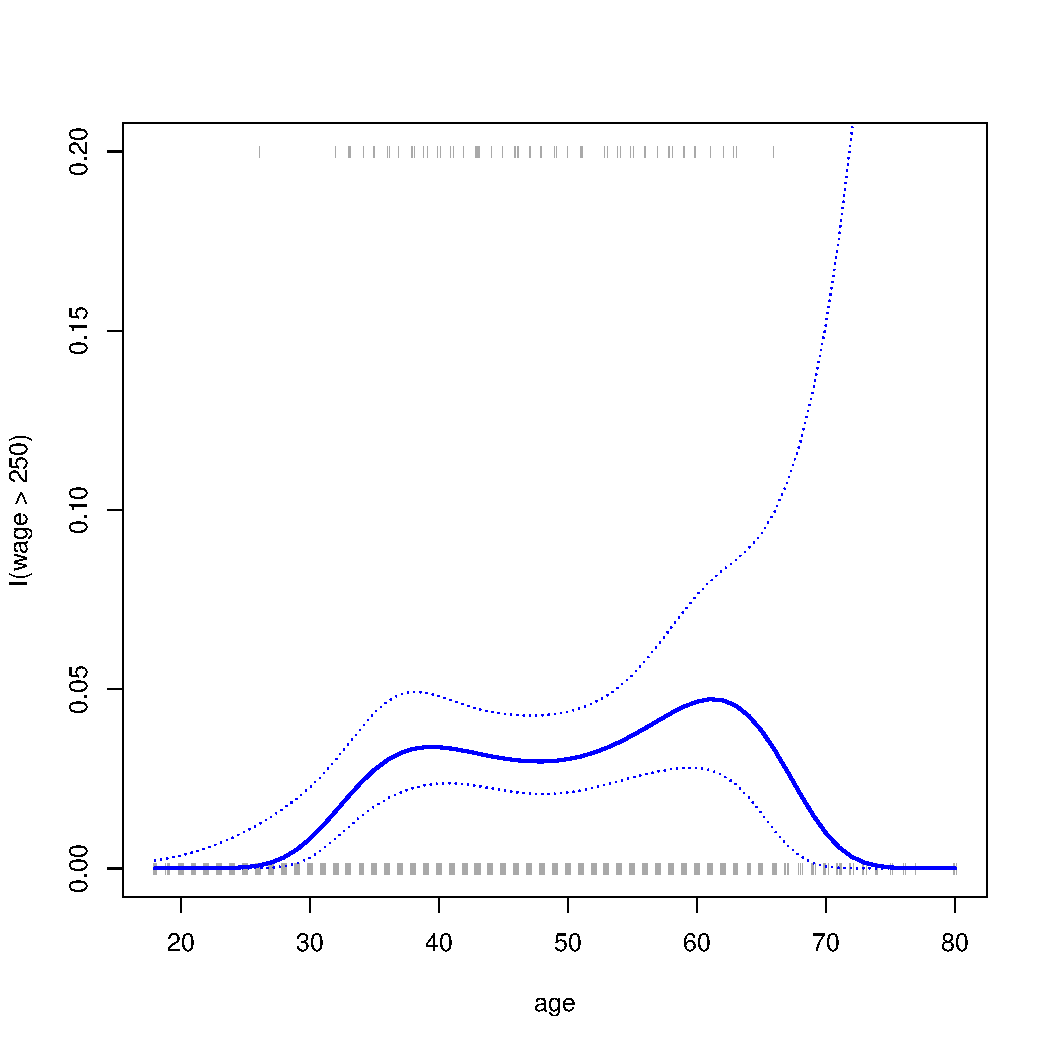
\includegraphics[width=\maxwidth]{figure/unnamed-chunk-15-1} 

\end{knitrout}

In order to fit a step function, as discussed in Section 7.2, we use the \texttt{cut()} function.

\begin{knitrout}
\definecolor{shadecolor}{rgb}{0.969, 0.969, 0.969}\color{fgcolor}\begin{kframe}
\begin{alltt}
\hlkwd{table}\hlstd{(}\hlkwd{cut}\hlstd{(age,}\hlnum{4}\hlstd{))}
\end{alltt}
\begin{verbatim}
## 
## (17.9,33.5]   (33.5,49]   (49,64.5] (64.5,80.1] 
##         750        1399         779          72
\end{verbatim}
\begin{alltt}
\hlstd{fit}\hlkwb{=}\hlkwd{lm}\hlstd{(wage}\hlopt{~}\hlkwd{cut}\hlstd{(age,}\hlnum{4}\hlstd{),} \hlkwc{data} \hlstd{= Wage)}
\hlkwd{coef}\hlstd{(}\hlkwd{summary}\hlstd{(fit))}
\end{alltt}
\begin{verbatim}
##                         Estimate Std. Error   t value     Pr(>|t|)
## (Intercept)            94.158392   1.476069 63.789970 0.000000e+00
## cut(age, 4)(33.5,49]   24.053491   1.829431 13.148074 1.982315e-38
## cut(age, 4)(49,64.5]   23.664559   2.067958 11.443444 1.040750e-29
## cut(age, 4)(64.5,80.1]  7.640592   4.987424  1.531972 1.256350e-01
\end{verbatim}
\end{kframe}
\end{knitrout}

Here \texttt{cut()} automatically picked the cutpoints at 33.5, 49, and 64.5 years of age. The function \texttt{cut()} returns an ordered categorical variable; the \texttt{lm()} function then creates a set of dummy variables for use in the regression. The \texttt{age<33.5} category is left out, so the intercept coefficient of \$94,160 can be interpreted as the average salary for those under 33.5 years of age, and the other coefficients can be interpreted as the average additional salary for those in the other age groups.\\

We can produce predictions and plots just as we did in the case of the polynomial fit:
\begin{knitrout}
\definecolor{shadecolor}{rgb}{0.969, 0.969, 0.969}\color{fgcolor}\begin{kframe}
\begin{alltt}
\hlstd{preds}\hlkwb{=}\hlkwd{predict}\hlstd{(fit,} \hlkwc{newdata}\hlstd{=}\hlkwd{list}\hlstd{(}\hlkwc{age}\hlstd{=age.grid),} \hlkwc{se}\hlstd{=}\hlnum{TRUE}\hlstd{)}
\hlstd{se.bands} \hlkwb{=} \hlkwd{cbind}\hlstd{(preds}\hlopt{$}\hlstd{fit}\hlopt{+}\hlnum{2}\hlopt{*}\hlstd{preds}\hlopt{$}\hlstd{se.fit, preds}\hlopt{$}\hlstd{fit}\hlopt{-}\hlnum{2}\hlopt{*}\hlstd{preds}\hlopt{$}\hlstd{se.fit)}

\hlkwd{plot}\hlstd{(age, wage,} \hlkwc{xlim}\hlstd{=agelims,} \hlkwc{cex}\hlstd{=}\hlnum{.5}\hlstd{,} \hlkwc{col}\hlstd{=}\hlstr{"darkgrey"}\hlstd{)}
\hlkwd{title}\hlstd{(}\hlstr{"Step Function"}\hlstd{,} \hlkwc{outer}\hlstd{=T)}
\hlkwd{lines}\hlstd{(age.grid, preds}\hlopt{$}\hlstd{fit,} \hlkwc{lwd}\hlstd{=}\hlnum{2}\hlstd{,} \hlkwc{col}\hlstd{=}\hlstr{"blue"}\hlstd{)}
\hlkwd{matlines}\hlstd{(age.grid, se.bands,} \hlkwc{lwd}\hlstd{=}\hlnum{1}\hlstd{,} \hlkwc{col}\hlstd{=}\hlstr{"blue"}\hlstd{,} \hlkwc{lty}\hlstd{=}\hlnum{3}\hlstd{)}
\end{alltt}
\end{kframe}
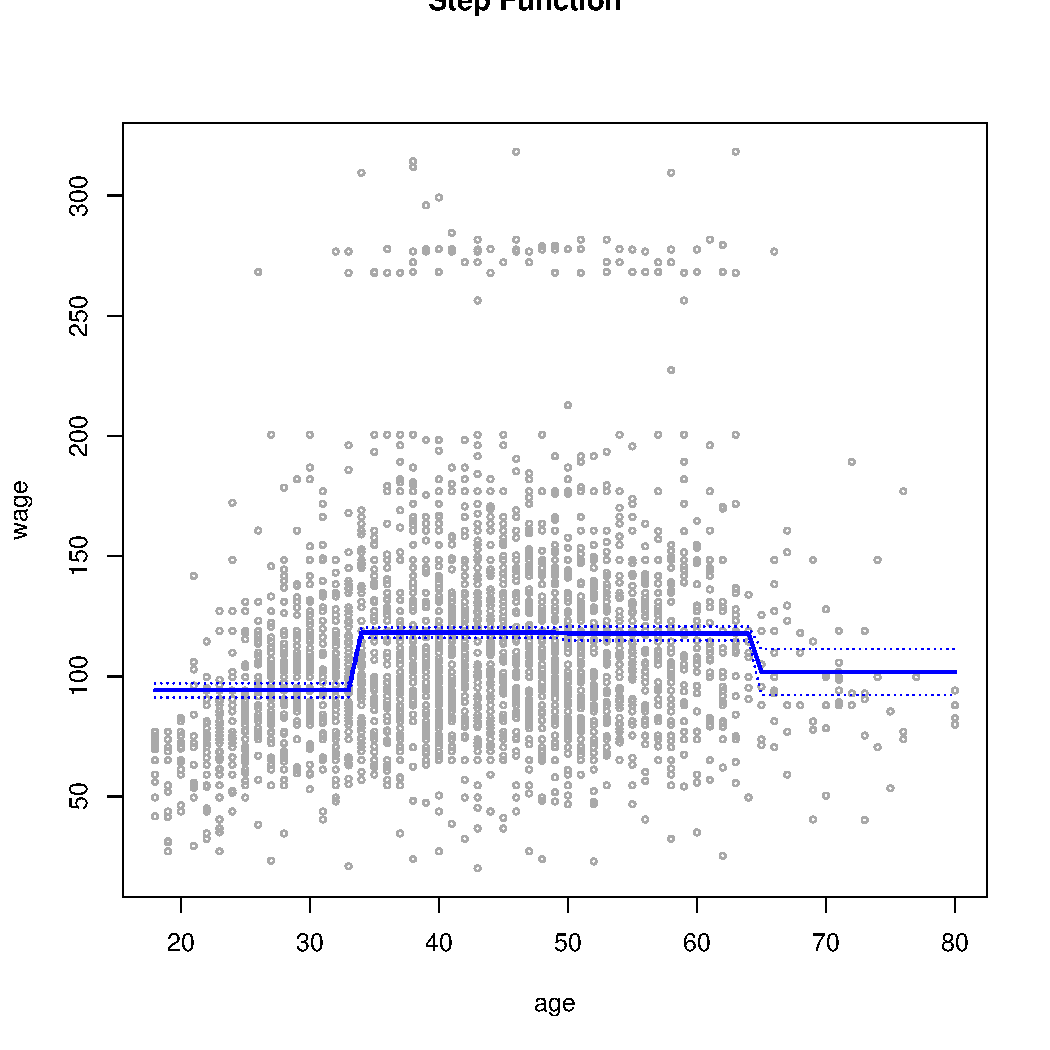
\includegraphics[width=\maxwidth]{figure/unnamed-chunk-17-1} 

\end{knitrout}

\newpage
\section{Splines}

\section{GAMs}


\end{document}
